% python classes slides - classes
% (c) 2012 Kostiantyn Danylov aka koder 
% koder.mail@gmail.com
% distributed under CC-BY licence
% http://creativecommons.org/licenses/by/3.0/deed.en

\documentclass{article}
% XeLaTeX
\usepackage{xltxtra}
\usepackage{xunicode}
\usepackage{listings}
\usepackage[landscape]{geometry}

% Fonts
\setmainfont{DejaVu Sans} %{Arial}
\newfontfamily\cyrillicfont{Nimbus Roman No9 L} %{Arial}
\setmonofont{Courier New}
%\setmonofont{Ubuntu Mono}

%\setmonofont{DejaVu Sans Mono}

% Lang
\usepackage{polyglossia}
\setmainlanguage{russian}
\setotherlanguage{english}
\usepackage[dvipsnames,table]{xcolor}


\ifx\pdfoutput\undefined
\usepackage{graphicx}
\else
\usepackage[pdftex]{graphicx}
\fi

\lstset{
	language=python,
	keywordstyle=\color{Emerald},%\texttt, 
	commentstyle=\color{OliveGreen},%\texttt,
	stringstyle=\color{Bittersweet},%\texttt,
	tabsize=4,
	numbers=left,
	xleftmargin=10pt,
	morekeywords={with,as},	
	numberstyle=\large,
	%identifierstyle=\texttt,
	%basicstyle=\texttt,
}

\usepackage{hyperref}

\hypersetup{
	colorlinks=true,
	urlcolor=blue
}

\usepackage{float}
%\floatstyle{boxed} 
%\restylefloat{figure}
\usepackage[normalem]{ulem}


\makeatletter
\def\PY@reset{\let\PY@it=\relax \let\PY@bf=\relax%
    \let\PY@ul=\relax \let\PY@tc=\relax%
    \let\PY@bc=\relax \let\PY@ff=\relax}
\def\PY@tok#1{\csname PY@tok@#1\endcsname}
\def\PY@toks#1+{\ifx\relax#1\empty\else%
    \PY@tok{#1}\expandafter\PY@toks\fi}
\def\PY@do#1{\PY@bc{\PY@tc{\PY@ul{%
    \PY@it{\PY@bf{\PY@ff{#1}}}}}}}
\def\PY#1#2{\PY@reset\PY@toks#1+\relax+\PY@do{#2}}

\expandafter\def\csname PY@tok@gd\endcsname{\def\PY@tc##1{\textcolor[rgb]{0.63,0.00,0.00}{##1}}}
\expandafter\def\csname PY@tok@gu\endcsname{\let\PY@bf=\textbf\def\PY@tc##1{\textcolor[rgb]{0.50,0.00,0.50}{##1}}}
\expandafter\def\csname PY@tok@gt\endcsname{\def\PY@tc##1{\textcolor[rgb]{0.00,0.25,0.82}{##1}}}
\expandafter\def\csname PY@tok@gs\endcsname{\let\PY@bf=\textbf}
\expandafter\def\csname PY@tok@gr\endcsname{\def\PY@tc##1{\textcolor[rgb]{1.00,0.00,0.00}{##1}}}
\expandafter\def\csname PY@tok@cm\endcsname{\let\PY@it=\textit\def\PY@tc##1{\textcolor[rgb]{0.25,0.50,0.50}{##1}}}
\expandafter\def\csname PY@tok@vg\endcsname{\def\PY@tc##1{\textcolor[rgb]{0.10,0.09,0.49}{##1}}}
\expandafter\def\csname PY@tok@m\endcsname{\def\PY@tc##1{\textcolor[rgb]{0.40,0.40,0.40}{##1}}}
\expandafter\def\csname PY@tok@mh\endcsname{\def\PY@tc##1{\textcolor[rgb]{0.40,0.40,0.40}{##1}}}
\expandafter\def\csname PY@tok@go\endcsname{\def\PY@tc##1{\textcolor[rgb]{0.50,0.50,0.50}{##1}}}
\expandafter\def\csname PY@tok@ge\endcsname{\let\PY@it=\textit}
\expandafter\def\csname PY@tok@vc\endcsname{\def\PY@tc##1{\textcolor[rgb]{0.10,0.09,0.49}{##1}}}
\expandafter\def\csname PY@tok@il\endcsname{\def\PY@tc##1{\textcolor[rgb]{0.40,0.40,0.40}{##1}}}
\expandafter\def\csname PY@tok@cs\endcsname{\let\PY@it=\textit\def\PY@tc##1{\textcolor[rgb]{0.25,0.50,0.50}{##1}}}
\expandafter\def\csname PY@tok@cp\endcsname{\def\PY@tc##1{\textcolor[rgb]{0.74,0.48,0.00}{##1}}}
\expandafter\def\csname PY@tok@gi\endcsname{\def\PY@tc##1{\textcolor[rgb]{0.00,0.63,0.00}{##1}}}
\expandafter\def\csname PY@tok@gh\endcsname{\let\PY@bf=\textbf\def\PY@tc##1{\textcolor[rgb]{0.00,0.00,0.50}{##1}}}
\expandafter\def\csname PY@tok@ni\endcsname{\let\PY@bf=\textbf\def\PY@tc##1{\textcolor[rgb]{0.60,0.60,0.60}{##1}}}
\expandafter\def\csname PY@tok@nl\endcsname{\def\PY@tc##1{\textcolor[rgb]{0.63,0.63,0.00}{##1}}}
\expandafter\def\csname PY@tok@nn\endcsname{\let\PY@bf=\textbf\def\PY@tc##1{\textcolor[rgb]{0.00,0.00,1.00}{##1}}}
\expandafter\def\csname PY@tok@no\endcsname{\def\PY@tc##1{\textcolor[rgb]{0.53,0.00,0.00}{##1}}}
\expandafter\def\csname PY@tok@na\endcsname{\def\PY@tc##1{\textcolor[rgb]{0.49,0.56,0.16}{##1}}}
\expandafter\def\csname PY@tok@nb\endcsname{\def\PY@tc##1{\textcolor[rgb]{0.00,0.50,0.00}{##1}}}
\expandafter\def\csname PY@tok@nc\endcsname{\let\PY@bf=\textbf\def\PY@tc##1{\textcolor[rgb]{0.00,0.00,1.00}{##1}}}
\expandafter\def\csname PY@tok@nd\endcsname{\def\PY@tc##1{\textcolor[rgb]{0.67,0.13,1.00}{##1}}}
\expandafter\def\csname PY@tok@ne\endcsname{\let\PY@bf=\textbf\def\PY@tc##1{\textcolor[rgb]{0.82,0.25,0.23}{##1}}}
\expandafter\def\csname PY@tok@nf\endcsname{\def\PY@tc##1{\textcolor[rgb]{0.00,0.00,1.00}{##1}}}
\expandafter\def\csname PY@tok@si\endcsname{\let\PY@bf=\textbf\def\PY@tc##1{\textcolor[rgb]{0.73,0.40,0.53}{##1}}}
\expandafter\def\csname PY@tok@s2\endcsname{\def\PY@tc##1{\textcolor[rgb]{0.73,0.13,0.13}{##1}}}
\expandafter\def\csname PY@tok@vi\endcsname{\def\PY@tc##1{\textcolor[rgb]{0.10,0.09,0.49}{##1}}}
\expandafter\def\csname PY@tok@nt\endcsname{\let\PY@bf=\textbf\def\PY@tc##1{\textcolor[rgb]{0.00,0.50,0.00}{##1}}}
\expandafter\def\csname PY@tok@nv\endcsname{\def\PY@tc##1{\textcolor[rgb]{0.10,0.09,0.49}{##1}}}
\expandafter\def\csname PY@tok@s1\endcsname{\def\PY@tc##1{\textcolor[rgb]{0.73,0.13,0.13}{##1}}}
\expandafter\def\csname PY@tok@sh\endcsname{\def\PY@tc##1{\textcolor[rgb]{0.73,0.13,0.13}{##1}}}
\expandafter\def\csname PY@tok@sc\endcsname{\def\PY@tc##1{\textcolor[rgb]{0.73,0.13,0.13}{##1}}}
\expandafter\def\csname PY@tok@sx\endcsname{\def\PY@tc##1{\textcolor[rgb]{0.00,0.50,0.00}{##1}}}
\expandafter\def\csname PY@tok@bp\endcsname{\def\PY@tc##1{\textcolor[rgb]{0.00,0.50,0.00}{##1}}}
\expandafter\def\csname PY@tok@c1\endcsname{\let\PY@it=\textit\def\PY@tc##1{\textcolor[rgb]{0.25,0.50,0.50}{##1}}}
\expandafter\def\csname PY@tok@kc\endcsname{\let\PY@bf=\textbf\def\PY@tc##1{\textcolor[rgb]{0.00,0.50,0.00}{##1}}}
\expandafter\def\csname PY@tok@c\endcsname{\let\PY@it=\textit\def\PY@tc##1{\textcolor[rgb]{0.25,0.50,0.50}{##1}}}
\expandafter\def\csname PY@tok@mf\endcsname{\def\PY@tc##1{\textcolor[rgb]{0.40,0.40,0.40}{##1}}}
\expandafter\def\csname PY@tok@err\endcsname{\def\PY@bc##1{\setlength{\fboxsep}{0pt}\fcolorbox[rgb]{1.00,0.00,0.00}{1,1,1}{\strut ##1}}}
\expandafter\def\csname PY@tok@kd\endcsname{\let\PY@bf=\textbf\def\PY@tc##1{\textcolor[rgb]{0.00,0.50,0.00}{##1}}}
\expandafter\def\csname PY@tok@ss\endcsname{\def\PY@tc##1{\textcolor[rgb]{0.10,0.09,0.49}{##1}}}
\expandafter\def\csname PY@tok@sr\endcsname{\def\PY@tc##1{\textcolor[rgb]{0.73,0.40,0.53}{##1}}}
\expandafter\def\csname PY@tok@mo\endcsname{\def\PY@tc##1{\textcolor[rgb]{0.40,0.40,0.40}{##1}}}
\expandafter\def\csname PY@tok@kn\endcsname{\let\PY@bf=\textbf\def\PY@tc##1{\textcolor[rgb]{0.00,0.50,0.00}{##1}}}
\expandafter\def\csname PY@tok@mi\endcsname{\def\PY@tc##1{\textcolor[rgb]{0.40,0.40,0.40}{##1}}}
\expandafter\def\csname PY@tok@gp\endcsname{\let\PY@bf=\textbf\def\PY@tc##1{\textcolor[rgb]{0.00,0.00,0.50}{##1}}}
\expandafter\def\csname PY@tok@o\endcsname{\def\PY@tc##1{\textcolor[rgb]{0.40,0.40,0.40}{##1}}}
\expandafter\def\csname PY@tok@kr\endcsname{\let\PY@bf=\textbf\def\PY@tc##1{\textcolor[rgb]{0.00,0.50,0.00}{##1}}}
\expandafter\def\csname PY@tok@s\endcsname{\def\PY@tc##1{\textcolor[rgb]{0.73,0.13,0.13}{##1}}}
\expandafter\def\csname PY@tok@kp\endcsname{\def\PY@tc##1{\textcolor[rgb]{0.00,0.50,0.00}{##1}}}
\expandafter\def\csname PY@tok@w\endcsname{\def\PY@tc##1{\textcolor[rgb]{0.73,0.73,0.73}{##1}}}
\expandafter\def\csname PY@tok@kt\endcsname{\def\PY@tc##1{\textcolor[rgb]{0.69,0.00,0.25}{##1}}}
\expandafter\def\csname PY@tok@ow\endcsname{\let\PY@bf=\textbf\def\PY@tc##1{\textcolor[rgb]{0.67,0.13,1.00}{##1}}}
\expandafter\def\csname PY@tok@sb\endcsname{\def\PY@tc##1{\textcolor[rgb]{0.73,0.13,0.13}{##1}}}
\expandafter\def\csname PY@tok@k\endcsname{\let\PY@bf=\textbf\def\PY@tc##1{\textcolor[rgb]{0.00,0.50,0.00}{##1}}}
\expandafter\def\csname PY@tok@se\endcsname{\let\PY@bf=\textbf\def\PY@tc##1{\textcolor[rgb]{0.73,0.40,0.13}{##1}}}
\expandafter\def\csname PY@tok@sd\endcsname{\let\PY@it=\textit\def\PY@tc##1{\textcolor[rgb]{0.73,0.13,0.13}{##1}}}

\def\PYZbs{\char`\\}
\def\PYZus{\char`\_}
\def\PYZob{\char`\{}
\def\PYZcb{\char`\}}
\def\PYZca{\char`\^}
\def\PYZam{\char`\&}
\def\PYZlt{\char`\<}
\def\PYZgt{\char`\>}
\def\PYZsh{\char`\#}
\def\PYZpc{\char`\%}
\def\PYZdl{\char`\$}
\def\PYZti{\char`\~}
% for compatibility with earlier versions
\def\PYZat{@}
\def\PYZlb{[}
\def\PYZrb{]}
\makeatother

\begin{document}
\LARGE

%-------------------------------------------------------------------------------
\begin{center} Класс \end{center}
\begin{itemize}
    \item Класс - это тип данных.
    \item Он содержит методы, работающие над объектами
    \item Объекты - экземпляры класса. Они хранят данные, используемые методами
    \item Данные должны быть взаимосвязанны, а функции формировать API, 
            достаточной для полноценной работы над данными   \sout{без прямого 
            доступа к ним}
    \item Структура класса чаще всего должна отображать структуру задачи
    \item Язык обеспечивает автоматизацию многих задач по поддержке ООП
\end{itemize}
\newpage

%-------------------------------------------------------------------------------
\begin{center} Объект и инстанцирование \end{center}
\begin{itemize}
    \item Объект - экземпляр класса. Хранилище данных.
    \item Объект получается путем инстанцирования класса. 
          В питоне инстанцирование это вызов
               \lstinline!obj = Class(...)!
    \item Одновременно может существовать неограниченное количество 
          экземпляров класса, все они независимы
\end{itemize}
\newpage

%-------------------------------------------------------------------------------
\begin{center} Интерфейсы \end{center}
\begin{itemize}
    \item Интерфейс - это логически взаимосвязанный набор операций, 
          которые можно проделать над типом
          Например файл - это интерфейс. Из него можно читать, в него можно писать.
    \item Классы реализуют интерфейсы
    \item Экземпляры классов предоставляют интерфейсы
    \item Класс может реализовывать множество интерфейсов
    \item Вообще в питоне интерфейсы используются редко, 
          так как плохо совместимы с утиной типизацией (но см. модуль ABС)
\end{itemize}
\newpage

%-------------------------------------------------------------------------------
\begin{center} 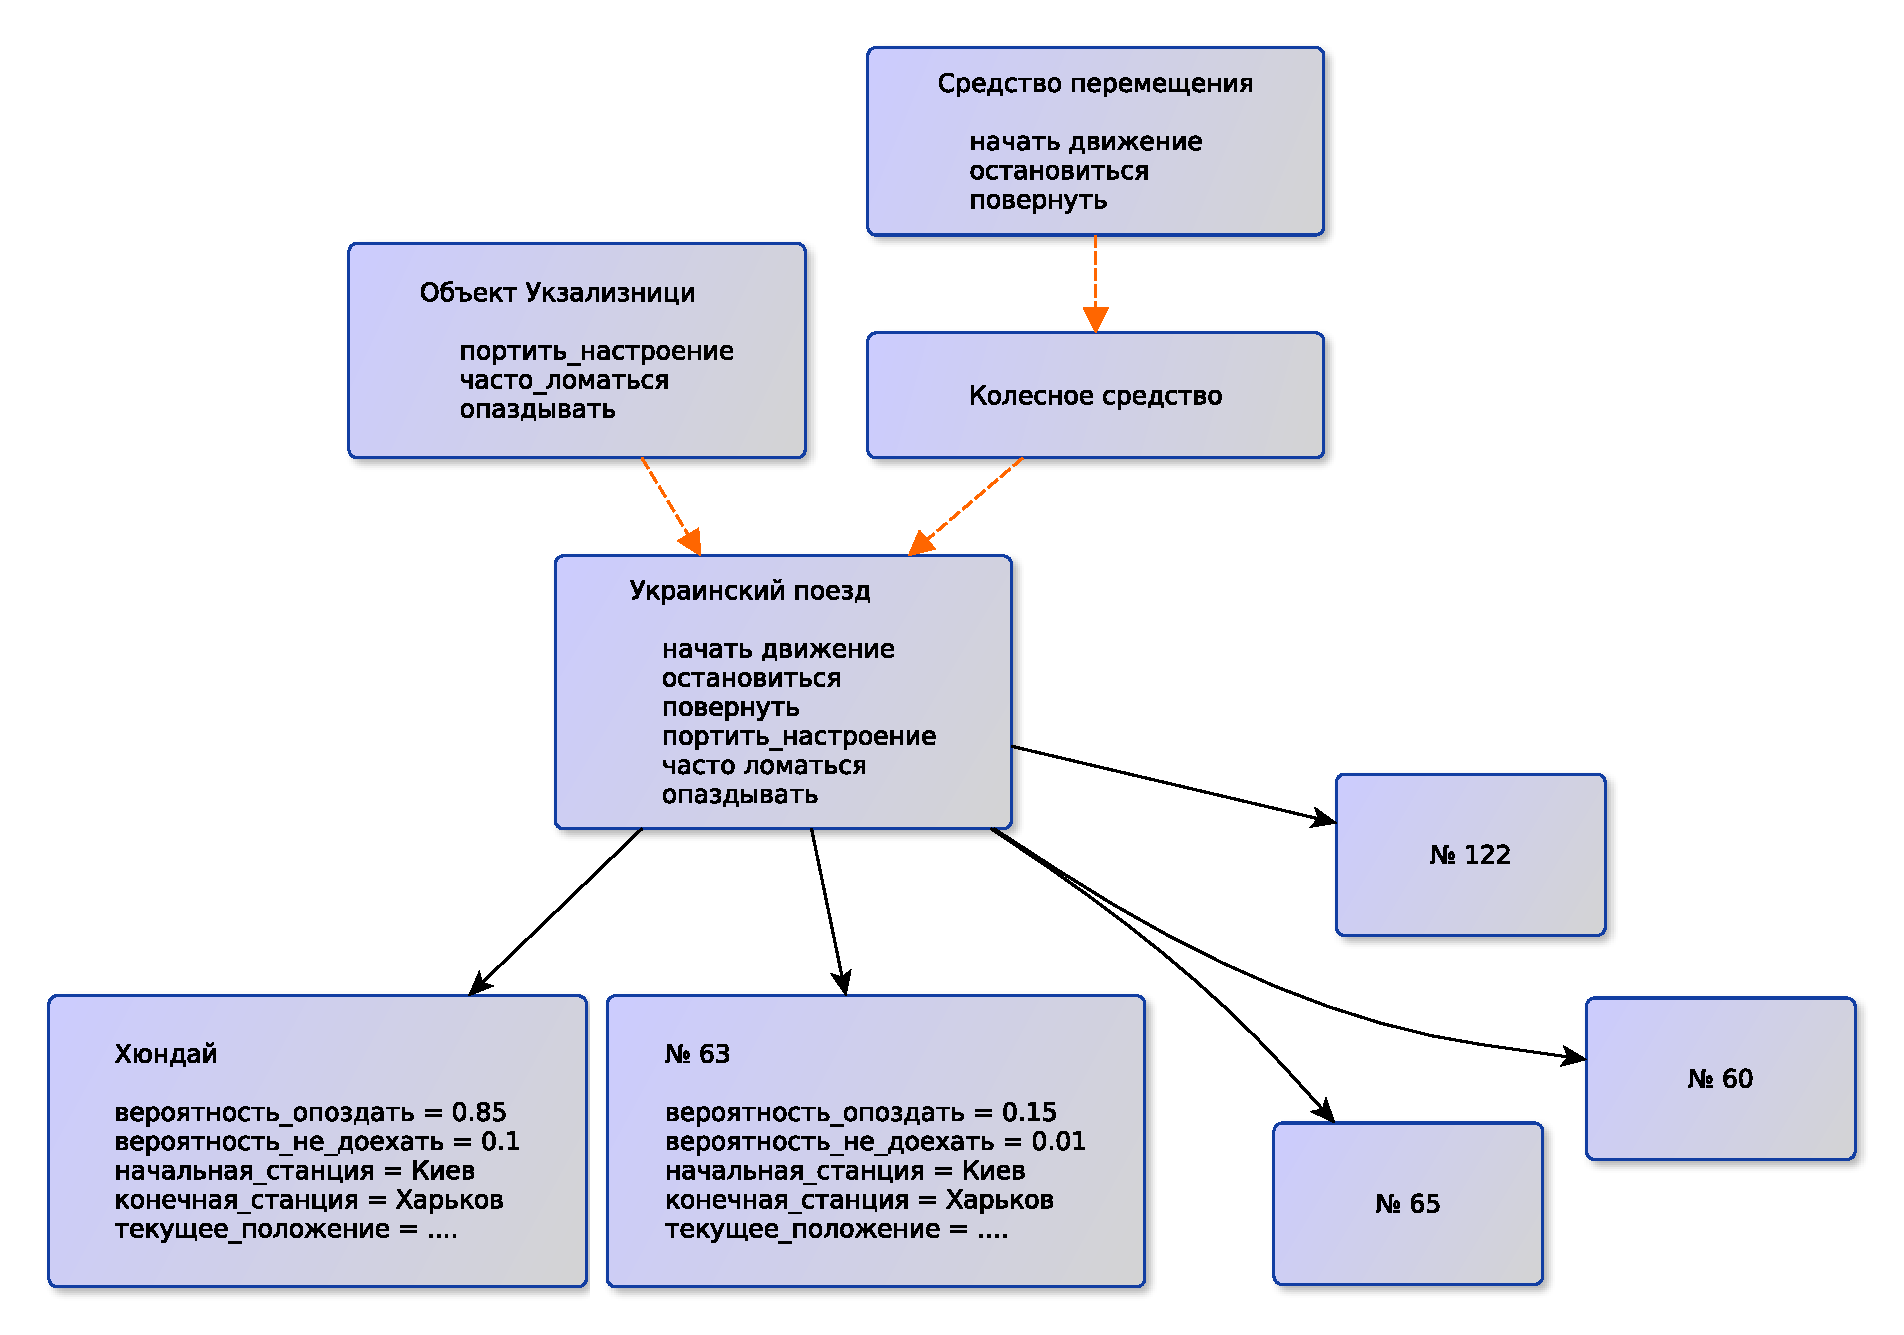
\includegraphics[scale=0.8]{images/ukr_zalilnitsya.eps} \end{center}
\newpage

%-------------------------------------------------------------------------------
\begin{center} Пример класса на python \end{center}
\vspace{15pt}
\begin{lstlisting}
    class Simple(object):
        "class documentation"
        def set_power(self, power):
            self.power = power

        def method(self, val):
            "method documentation"
            return val ** self.power

    simple = Simple()
    simple.set_power(1.0 / 3)
    simple.method(8) == 2.0  # not the best idea, but works
\end{lstlisting}
\newpage

%-------------------------------------------------------------------------------
\begin{center} Поля класса \end{center}
\begin{itemize}
    \item Поля это переменные, связанные с экземпляром класса
    \item Класс явно не определяет какие поля будут у его объектов
    \item У каждого экзампляра они свои
    \item Доступ производится с помошью оператора '.'
    \item Как и переменные они создаются присваиванием
    \item = Можно динамически создавать/удалять поля у объекта
    \item = Разные экземпляры могут иметь разные наборы полей
    \item Предыдущие два пункта чаще всего - пример плохого поведения
\end{itemize}
\begin{lstlisting}
    simple = Simple()
    simple.a = 12
    print simple.a
    simple.a += 4
\end{lstlisting}
\newpage

%-------------------------------------------------------------------------------
\begin{center} Методы класса\end{center}
\begin{itemize}
    \item Методы это функции, объявленные внутри тела класса
    \item Должны вызываться только от экземпляра класса
    \item Первым параметром метод автоматически получает экзампляр, от которого вызван
\end{itemize}

\begin{lstlisting}
    Simple.method(12) # ошибка
    simple = Simple()
    simple.method(12) == Simple.method(simple, 12)
\end{lstlisting}
\newpage

%-------------------------------------------------------------------------------
\begin{center} Нет инкапсуляции \end{center}
\begin{itemize}
    \item "Принцип открытого кимоно" == 
        "мы не знаем как совместить инкапсуляцию 
        с остальными возможностями языка"
    \item Есть property, "скрытые поля" (но они предназначенны для другого)
    \item В отличии от Java всегда можно изменить поле на свойство 
            с сохранением совместимости
    \item Можно реализовать любой вид инкапсуляции динамической
    \item Ничего из этого не получило какого-нить распространения в питоне
    \item Документирование API vs чтение заголовков
    \item Реализуя сокрытие полей объекта вы 
        создаете проблемы многим библиотекам python
\end{itemize}
\newpage

%-------------------------------------------------------------------------------
\begin{center} Наследование \end{center}
\begin{itemize}
    \item У класса может быть один или несколько родительских классов, 
          класс автоматически получает все методы, которые были у его родителей
          и может добавить дополнительные
    \item Поддерживается множественное наследование
    \item Которое не надо использовать, если на то нет существенных причин
\end{itemize}

{
\Large
\vspace{15pt}
\begin{lstlisting}
    class A(object):
        def some_method(self):
            print "A.some_meth"

    class B(A):
        def some_method2(self):
            print "B.some_meth2"

    b = B() 
    b.some_method2() # B.some_method2 called
    b.some_method() # A.some_meth called
\end{lstlisting}
}
\newpage

%-------------------------------------------------------------------------------
\begin{center} Полиморфизм \end{center}
\begin{itemize}
    \item Наследник может изменить поведение методов предка
    \item Все методы - виртуальные
\end{itemize}
{
\Large
\vspace{15pt}
\begin{lstlisting}
    class A(object):
        def some_method(self):
            print "A.some_meth"

    class B(A):
        def some_method(self):
            print "B.some_meth"

    a = A() 
    a.some_method() # A.some_meth

    b = B() 
    b.some_method() # B.some_meth
\end{lstlisting}
}
\newpage

%-------------------------------------------------------------------------------
\begin{center} Вызов метода базового класса \end{center}
\vspace{15pt}
\begin{lstlisting}
    class A(object):
        def some_method(self, val):
            print "A.some_method({!r})".format(val)

    class B(A):
        def some_method(self, val):
            print "B.some_method({!r})".format(val)
            A.some_method(self, val)

    b = B() 
    b.some_method(1)
    # B.some_method(1)
    # A.some_method(1)
\end{lstlisting}
\newpage

%-------------------------------------------------------------------------------
\begin{center} super \end{center}
\begin{itemize}
    \item Прямой метод хорошо работает при одиночном наследовании
    \item super(CurrentClass, self).method позволяет корректно вызывать 
            метод у базового класса
    \item Даже в случае множественного наследования вызывать super нужно только один раз
    \item super использует линеаризацию - упорядочивание иерархии базовых классов в последовательность
    \item \href{http://www.python.org/download/releases/2.3/mro/}{Подробное описание линеаризации}.
\end{itemize}
\newpage

%-------------------------------------------------------------------------------
\begin{center} Прямой вызов при множественном наследовании \end{center}
\begin{lstlisting}
    class A(object):
        def draw(self, pt):
            some_action(pt)

    class B(A):
        def draw(self, pt):
            A.draw(pt)

    class C(A):
        def draw(self, pt):
            A.draw(pt)

    class D(C, B):
        def draw(self, pt):
            C.draw(pt)
            B.draw(pt)
\end{lstlisting}
\newpage

%-------------------------------------------------------------------------------
\begin{center} super при множественном наследовании \end{center}
\begin{lstlisting}
    class A(object):
        def draw(self, pt):
            some_action(pt)

    class B(A):
        def draw(self, pt):
            super(B, self).draw(pt)

    class C(A):
        def draw(self, pt):
            super(C, self).draw(pt)

    class D(C, B):
        def draw(self, pt):
            super(D, self).draw(pt)
\end{lstlisting}
\newpage

%-------------------------------------------------------------------------------
\begin{center}direct call VS super\end{center}
\begin{center} 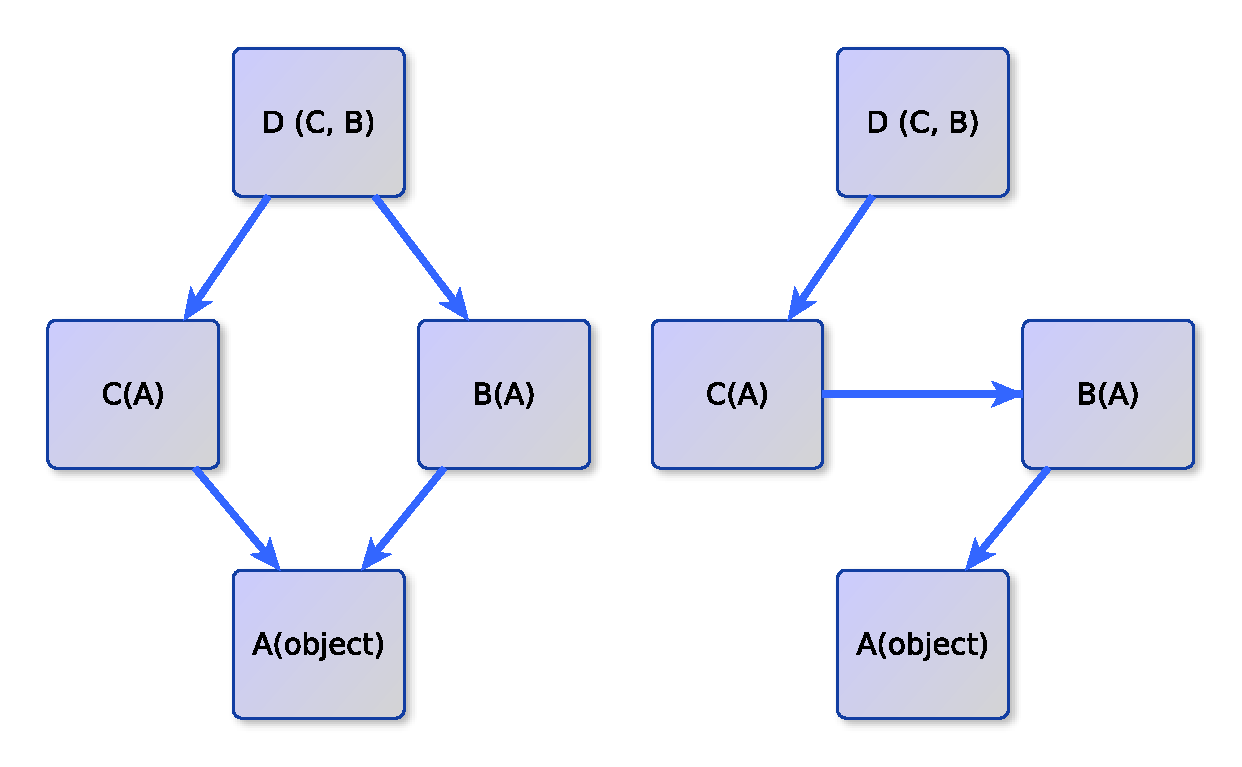
\includegraphics{images/linearization_simple.eps} \end{center} 
\newpage

%-------------------------------------------------------------------------------
\begin{center}Пример линеаризации\end{center}
\begin{center} 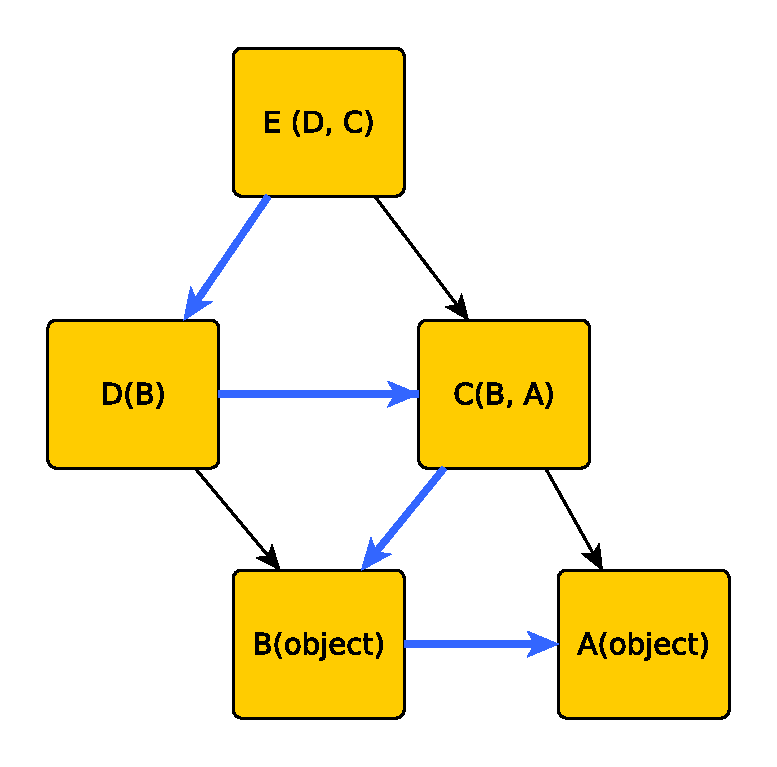
\includegraphics{images/inheritance_1.eps} \end{center} 
\newpage

%-------------------------------------------------------------------------------
\begin{center}Пример линеаризации 2\end{center}
\begin{center} 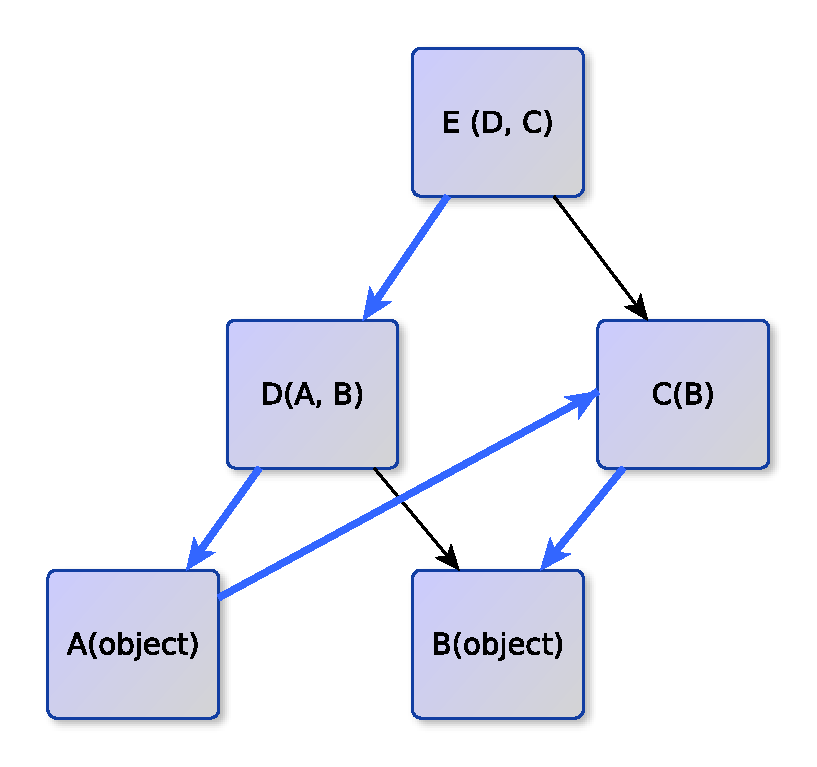
\includegraphics{images/inheritance_2.eps} \end{center} 
\newpage

%-------------------------------------------------------------------------------
\begin{center}Нелинеаризуемая иерархия классов\end{center}
\begin{center} 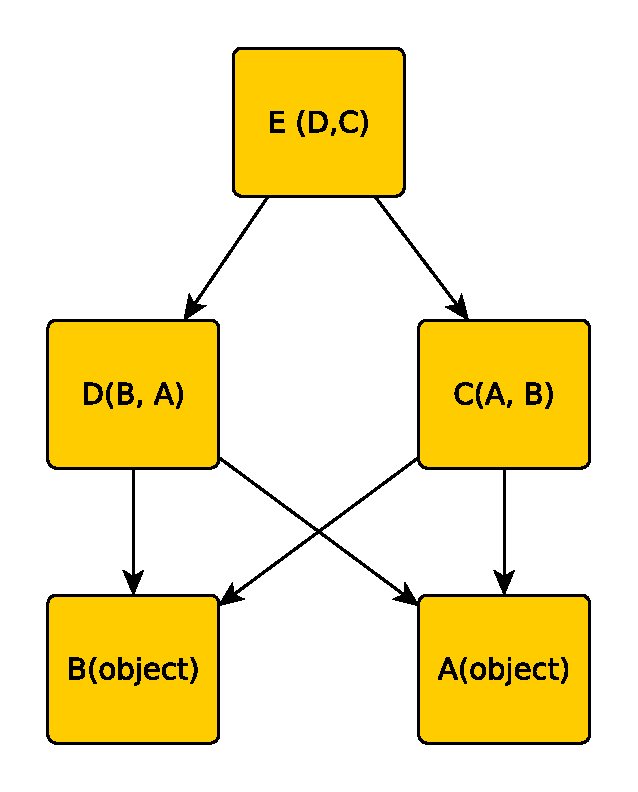
\includegraphics{images/linearization_fail.eps} \end{center} 
\newpage

%-------------------------------------------------------------------------------
\begin{center}Ошибки при построении иерархии\end{center}
Если имена совпали случайно, то нельзя использовать super в E \\
\begin{center} 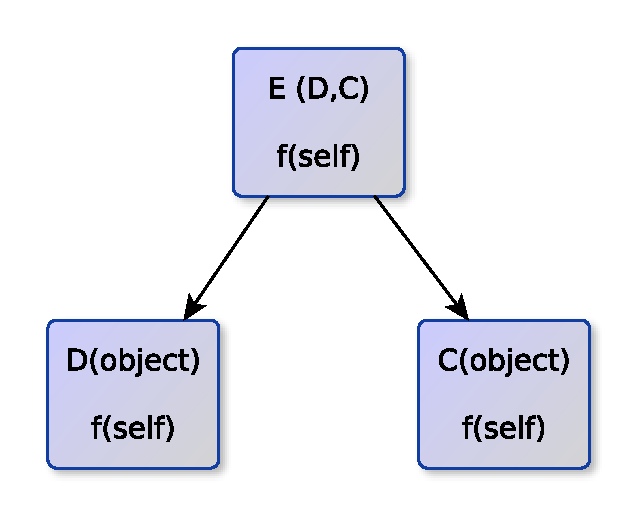
\includegraphics[scale=0.9]{images/missed_base_class.eps} \end{center}
\newpage

%-------------------------------------------------------------------------------
\begin{center}Ошибки при построении иерархии\end{center}
Если имена совпали не случайно, то нужно добавить базовый класс и super будет работать нормально\\
\begin{center} 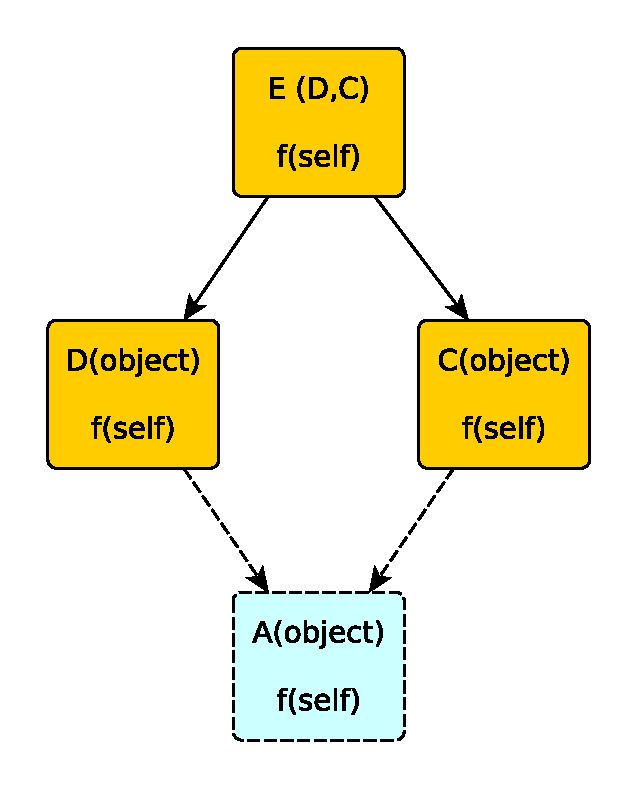
\includegraphics[scale=0.9]{images/missed_base_class_2.eps} \end{center}
\newpage

%-------------------------------------------------------------------------------
\begin{center} Конструктор \lstinline!__init__! \end{center}
\begin{itemize}
    \item \lstinline!__init__!(конструктор) - метод, который автоматически вызывается 
        при создании экземпляра класса и должен его проинициализировать - 
        присвоить всем переменным начальные значения.
    \item К сожалению \_\_init\_\_ это типичный пример ошибки
\end{itemize}
\vspace{15pt}
\begin{lstlisting}
    class A(object):
        def __init__(self, val):
            self.msg = "val = {}".format(val)
            print "A inited with value", val

    a = A(1) # A inited with value 1
    print a.msg # val = 1
\end{lstlisting}
\newpage

%-------------------------------------------------------------------------------
\begin{center} Деструктор \lstinline!__del__! \end{center}
\begin{itemize}
    \item \lstinline!__del__! должен вызываться перед удалением объекта 
        (и, обычно, вызывается).
    \item Если нет циклических ссылок
    \item Или объект не попал во фрейм, где произошла ошибка
    \item Правильно - использовать with вместо надежд на \_\_del\_\_
    \item \lstinline!def __del__(self):...!
\end{itemize}
\newpage

%-------------------------------------------------------------------------------
%level=3
\begin{center} Аллокатор \lstinline!__new__! \end{center}
\begin{itemize}
    \item \lstinline!__new__! аналог перегрузки new в С++
    \item Классовый метод(автоматически), вызываемый для создания 
        нового экземпляра объекта, который затем будет проинициализирован 
        с помощью \lstinline!__init__!. classmethod использовать не надо.
    \item Получает те-же параметры, что и \lstinline!__init__!.
\end{itemize}
\newpage
%-------------------------------------------------------------------------------
\begin{center} Аллокатор \lstinline!__new__! \end{center}
\begin{lstlisting}
    class X(object):
        def __new__(cls, val):
            print "{}.__new__({!r})".format(
                    cls.__name__, val)
            return object.__new__(cls, val)
        
        def __init__(self, val):
            print "{}.__init__({!r})".format(
                    self.__class__.__name__, val)

    X(1)
    #X.__new__(1)
    #X.__init__(1)
\end{lstlisting}
\newpage

%-------------------------------------------------------------------------------
%level=3
\begin{center} Аллокатор \lstinline!__new__! \end{center}
\begin{itemize}
    \item \lstinline!__new__! может вернуть объект другого типа
    \item Наверное, не самая лучшая идея
\end{itemize}
\vspace{15pt}
\begin{lstlisting}
    class A(object):
        def __init__(self, x):
            pass

    class B(object):
        def __init__(self, x, y):
            pass
        def __new__(cls, x, y=None):
            if y is None:
                return A(x)
            else:
                return super(B, cls).__new__(cls, x, y)

    print B(1, 2) #<__main__.B at 0x...>
    print B(1) # <__main__.A at 0x...>    
\end{lstlisting}
\newpage

%-------------------------------------------------------------------------------
\begin{center}isinstance, issubclass\end{center}
\begin{itemize}
    \item \lstinline!isinstance(x, Y)! - проверяет, что x экземпляр Y или
              одного из классов, наследованных от Y
    \item \lstinline!isinstance(x, (Y1, Y2, ..., YN))!
    \item \lstinline!issubclass(X, Y)! - проверяет, что X is Y или X
            прямо или косвенно раследует Y.
    \item \lstinline!issubclass(X, (Y1, Y2, ..., YN))!
\end{itemize}
\begin{lstlisting}
    isinstance(1, int) == True
    isinstance(2.0, int) == False
    isinstance("as", (str, unicode)) == True
    issubclass(int, int) == True
\end{lstlisting}
\newpage

%-------------------------------------------------------------------------------
%level=3
\begin{center} Скрытие полей \end{center}
\begin{itemize}
    \item \lstinline!__xxxx! - "скрытые поля и методы" 
        - переименовываются для избежания пересечения имен
    \item \lstinline!A.__xxx! -> \lstinline!A._A__xxx!
    \item Не для инкапсуляции
\end{itemize}
\newpage

%-------------------------------------------------------------------------------
\begin{center} Связанные и не связанные методы \end{center}
\begin{itemize}
    \item \lstinline!a = A(); a.b(1) == A.b(a, 1)!
    \item \lstinline!A.b! несвязанный метод. Требует получения экземпляра A первым параметром.
    \item \lstinline!A.b(1)! - ошибка. 
    \item \lstinline!(A.b)(a, 1)! - ok
    \item \lstinline!a.b! - связанный метод, эквивалентен функции.
\end{itemize}
\vspace{15pt}
\begin{lstlisting}
    a = A()
    t = a.b
    t(1) # a.b(1)
\end{lstlisting}
\newpage

%-------------------------------------------------------------------------------
\begin{center} Классовые и статические методы \end{center}
\begin{itemize}
    \item \lstinline!classmethod! превращяет метод в классовый, первым параметром вместо
          экземпляра такой метод получает класс и может быть вызван как от класса, 
          так и от экземпляра
    \item \lstinline!staticmethod! превращяет метод в статический (обычную функцию).
          может быть вызван как от класса, 
          так и от экземпляра
\end{itemize}
\newpage

%-------------------------------------------------------------------------------
\begin{center} Классовые и статические методы \end{center}
\begin{lstlisting}
    class A(object):
        val = 12

        @classmethod
        def meth1(cls, x):
            return x + cls.val

        @staticmethod
        def meth2(x, y):
            return x + y

    A.meth1(1) == 13
    A().meth2(1,2) == 3 

    class B(A):
        val = 13

    B.meth1(1) == 14
\end{lstlisting}
\newpage

%-------------------------------------------------------------------------------
\begin{center} Сортировка и сравнение \end{center}
\begin{itemize}
    \item По-умолчанию == для пользовательских классов использует is
    \item \lstinline!object_list.sort(cmp=lambda x,y : x.some_attr > y.some_attr)!
    \item \lstinline!object_list.sort(key=lambda x : x.some_attr)!
\end{itemize}
\newpage

%-------------------------------------------------------------------------------
\begin{center}Классы/объекты внутри\end{center}
\_\_dict\_\_, \_\_class\_\_, \_\_mro\_\_
\newpage

%-------------------------------------------------------------------------------

\begin{center}Задача\end{center}
Написать my\_super, которая работает, как встроенный super 
\newpage

%-------------------------------------------------------------------------------
\begin{center}присваивание классовым полям и полям экземпляра\end{center}
\newpage

%-------------------------------------------------------------------------------
property. ДЗ \_\_get\_\_, \_\_set\_\_, \_\_del\_\_
\newpage

%-------------------------------------------------------------------------------
\begin{center} Протоколы/перенругзка операторов \end{center}
\begin{center} int \end{center}
\begin{itemize}
    \item \lstinline!__add__(self, obj) # self + obj!
    \item \lstinline!__radd__(self, obj) #  obj + self!
    \item \lstinline!__iadd__(self, obj) #  self += obj!
    \item \lstinline!__int__(self) # int(self)!
\end{itemize}
\newpage

%-------------------------------------------------------------------------------
%level=TBD
\begin{center} Работа некоторых встроенных функций (протоколы встроенных функций) \end{center}
\begin{itemize}
    \item \lstinline!int(x) == x.__int__()!
    \item \lstinline!str(x) == x.__str__()!
    \item \lstinline!repr(x) == x.__repr__()!
    \item \lstinline!len(x) == x.__len__()!
    \item \lstinline!iter(x) == x.__iter__()!
    \item \lstinline!next(x) == x.next()! O\_o
    \item \lstinline!hex, oct, hash!
\end{itemize}
\newpage

%-------------------------------------------------------------------------------
% level=3
\begin{center} Специальные методы - контейнер \end{center}
\begin{itemize}
    \item \lstinline!x.__getitem__(index) # x[index]!
    \item \lstinline!x.__setitem__(index, val) # x[index] = val!
    \item \lstinline!x.__delitem__(index) # del x[index]!
    \item ...
\end{itemize}
\newpage

%-------------------------------------------------------------------------------
\begin{center} Специальные методы - доступ к атрибутам \end{center}
\begin{itemize}
    \item \lstinline!x.__getattribute__(name)!
    \item \lstinline!x.__getattr__(name)!
    \item \lstinline!x.__setattr__(name, val)!
    \item \lstinline!x.__delattr__(name)!
    \item \lstinline!getattr(x, name[, val])!
    \item \lstinline!setattr(x, name, val)!
    \item \lstinline!delattr(x, name)!
\end{itemize}
\newpage

%-------------------------------------------------------------------------------
\begin{center} Видео лекции \end{center}
	\href{http://www.youtube.com/watch?v=rDXuPBjVfSc&feature=related}{OOP Programming}
\newpage
%-------------------------------------------------------------------------------
\end{document}
